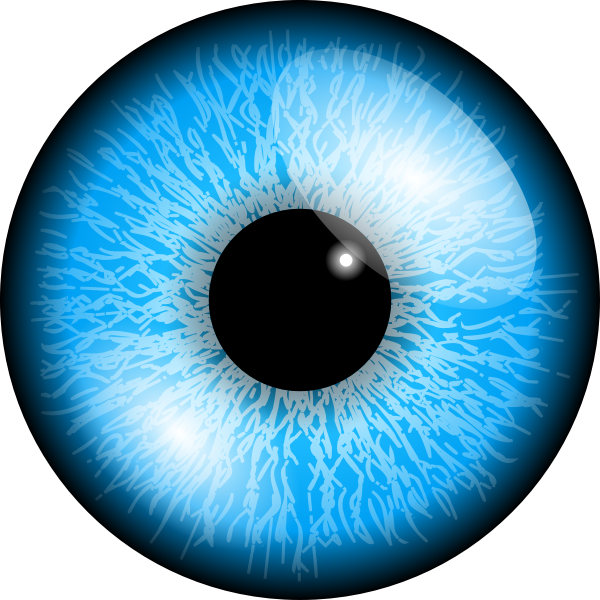
\includegraphics[height=1.5cm]{images/pictograms/visualisation}

\includegraphics[height=1.5cm]{images/pictograms/tools}


\lstinputlisting[language=bash,basicstyle=\small]{python_codes/fieldstone_97/keywords.key}

\begin{center}
Code at \url{https://github.com/cedrict/fieldstone/tree/master/python_codes/fieldstone_97}
\end{center}

\par\noindent\rule{\textwidth}{0.4pt}

%%%%%%%%%%%%%%%%%%%%%%%%%%%%%%%%%%%%%%%%%%%%%%%%%%%%%%%%%%%%%%%%%%%%%%%%%%%%%%%%%%%%%%%%

All CRUST 1.0 data are available at \url{https://igppweb.ucsd.edu/~gabi/crust1.html}. 
The files {\tt crust1.rho} and {\tt crust1.bnds} count 64,800 lines,
corresponding to 360x180 points, i.e. a 1\si{\degree} resolution. 

As explained on the website: 
"The model is defined from 89.5 to -89.5 deg latitude (so that 
in fact the data is the co-latitude) and -179.5 to 179.5 deg
longitude. Longitudes are the inner loop, i.e. all longitudes are stored
for each latitude, then the next latitude is given. The model starts at 
89.5 N and 179.5 W."

The structure of the CRUST 1.0 data is as follows:

\begin{verbatim}
===========================================================
 crust1.rho | layer | name             | crust1.bnds
 --------------------------------------|----0-------
 1          | 0     | water            |
 --------------------------------------|----1-------
 2          | 1     | ice              |
 --------------------------------------|----2-------
 3          | 2     | upper sediments  |
 --------------------------------------|----3-------
 4          | 3     | mid sediments    |
 --------------------------------------|----4-------
 5          | 4     | lower sediments  | 
 --------------------------------------|----5-------
 6          | 5     | upper crust      |
 --------------------------------------|----6-------
 7          | 6     | mid crust        |
 --------------------------------------|----7-------
 8          | 7     | lower crust      |
 --------------------------------------|----8-------MOHO
 9          | 8
===========================================================
\end{verbatim}

This stone allows the user to choose a minimum and maximum radius, as well as a 
number of shells in between {\tt nrad}, and rewrites the data in spherical coordinates 
as the ascii file {\tt crust1p0\_full\_for\_aspect.ascii} which is in the format that \aspect{} expects.
Another file, {\tt crust1p0\_moho\_for\_aspect.ascii}, is produced. Its structure and intent
is similar to the first one, except that points above the moho are assigned a single 
density $\rho=2900\si{\kilo\gram\per\cubic\metre}$ while points below the 
moho are assigned $\rho=3300\si{\kilo\gram\per\cubic\metre}$.

Very importantly, \aspect{} does not read in densities but temperatures. This stone then 
converts the density values into temperature using the simple relationship
\[
\rho = \rho_0 (1-\alpha(T-T_0))
\qquad \text{or,} \qquad
T= \frac{1}{\alpha} \left(1 - \frac{\rho}{\rho_0} \right)
\]
and we here take $\alpha = 3\cdot 10^{-5}\si{\per\kelvin}$, 
$T_0=0\si{\kelvin}$ and $\rho_0=3300\si{\kilo\gram\per\cubic\metre}$. 
This temperature is meaningless, but when used in the material model of \aspect{}, 
it yields the expected density field. 

CRUST 1.0 also comes with the file {\tt depthtomoho.xyz} which name is 
self-explanatory. Values are stored at coordinates $x.5$, $y.5$ (with $x\in[0,359]$
and $y\in [-89:89]$) so I assign a 1x1degree cell around it and give the whole cell 
the associated depth.
The data is exported as vtu file. One is a 2D lat-lon map (the vertical 
elevation of the map follows the moho depth) named {\tt moho\_map.vtu}, the other is a 
spherical mesh where each cell is assigned the radius of the Earth minus the moho depth, 
named {\tt moho\_shell.vtu}.

\begin{center}
\includegraphics[width=7.cm]{python_codes/fieldstone_97/images/mohodepth1}
\includegraphics[width=7.cm]{python_codes/fieldstone_97/images/mohodepth2}\\
\includegraphics[width=7.cm]{python_codes/fieldstone_97/images/mohodepth7}
\includegraphics[width=7.cm]{python_codes/fieldstone_97/images/mohodepth8}\\
\includegraphics[width=7.cm]{python_codes/fieldstone_97/images/mohodepth3}
\includegraphics[width=7.cm]{python_codes/fieldstone_97/images/mohodepth4}\\
\includegraphics[width=7.cm]{python_codes/fieldstone_97/images/mohodepth5}
\includegraphics[width=7.cm]{python_codes/fieldstone_97/images/mohodepth6}\\
\includegraphics[width=7.cm]{python_codes/fieldstone_97/images/mohodepth9}
\includegraphics[width=7.cm]{python_codes/fieldstone_97/images/mohodepth10}\\
{\captionfont colormap=vik, see \url{http://www.fabiocrameri.ch/vik.php}.
Continent boundaries are from Stone 69.}
\end{center}

\begin{center}
\includegraphics[width=5.cm]{python_codes/fieldstone_97/images/lat}
\includegraphics[width=5.cm]{python_codes/fieldstone_97/images/lon1}
\includegraphics[width=5.cm]{python_codes/fieldstone_97/images/lon2}\\
{\captionfont Note that latitudes start at 0 and go to 360, with 180
corresponding to Greenwich.}
\end{center}



Subsequently the code uses the same data, loops over each cell and assesses 
for each layer if it has non zero thickness. In this case it is added to 
the layer list. We find:

\begin{verbatim}
water      : 42549 cells out of 64800
ice        : 7550  cells out of 64800
up. seds.  : 60650 cells out of 64800
mid. seds. : 14355 cells out of 64800
low. seds. : 2471  cells out of 64800
up. crust  : 64800 cells out of 64800
mid. crust : 64800 cells out of 64800
low. crust : 64800 cells out of 64800
\end{verbatim}

From the lat-lon coordinates and the depths of the 
layer boundaries the coordinates of the 8 corners of the cell are 
computed and transformed into $x,y,z$ coordinates and exported to its 
respective vtu file (one per layer). These 8 files 
(water, ice, upper-middle-lower sediments and upper-middle-lower crust) are 
shown hereunder:

\begin{center}
\includegraphics[width=4.cm]{python_codes/fieldstone_97/images/layer00}
\includegraphics[width=4.cm]{python_codes/fieldstone_97/images/layer01}
\includegraphics[width=4.cm]{python_codes/fieldstone_97/images/layer02}
\includegraphics[width=4.cm]{python_codes/fieldstone_97/images/layer03}\\
\includegraphics[width=4.cm]{python_codes/fieldstone_97/images/layer04}
\includegraphics[width=4.cm]{python_codes/fieldstone_97/images/layer05}
\includegraphics[width=4.cm]{python_codes/fieldstone_97/images/layer06}
\includegraphics[width=4.cm]{python_codes/fieldstone_97/images/layer07}\\
{\captionfont 
From left to right, top to bottom, layers 0 to 7.
colormap=vik\footnote{\url{http://www.fabiocrameri.ch/vik.php}}.
Continent boundaries are from Stone 69.}
\end{center}

\begin{center}
\includegraphics[width=4.cm]{python_codes/fieldstone_97/images/thickness00}
\includegraphics[width=4.cm]{python_codes/fieldstone_97/images/thickness01}
\includegraphics[width=4.cm]{python_codes/fieldstone_97/images/thickness02}
\includegraphics[width=4.cm]{python_codes/fieldstone_97/images/thickness03}\\
\includegraphics[width=4.cm]{python_codes/fieldstone_97/images/thickness04}
\includegraphics[width=4.cm]{python_codes/fieldstone_97/images/thickness05}
\includegraphics[width=4.cm]{python_codes/fieldstone_97/images/thickness06}
\includegraphics[width=4.cm]{python_codes/fieldstone_97/images/thickness07}\\
{\captionfont 
From left to right, top to bottom, layers 0 to 7.
Continent boundaries are from Stone 69.}
\end{center}



\begin{center}
\includegraphics[width=4.cm]{python_codes/fieldstone_97/images/layer_area_00_rho}
\includegraphics[width=4.cm]{python_codes/fieldstone_97/images/layer_area_05_rho}
\includegraphics[width=4.cm]{python_codes/fieldstone_97/images/layer_area_06_rho}
\includegraphics[width=4.cm]{python_codes/fieldstone_97/images/layer_area_07_rho}\\
\includegraphics[width=4.cm]{python_codes/fieldstone_97/images/layer_area_00_thick}
\includegraphics[width=4.cm]{python_codes/fieldstone_97/images/layer_area_05_thick}
\includegraphics[width=4.cm]{python_codes/fieldstone_97/images/layer_area_06_thick}
\includegraphics[width=4.cm]{python_codes/fieldstone_97/images/layer_area_07_thick}\\
{\captionfont Water, upper, middle and lower crust layers, for longitudes between
60+180 and 100+180 and latitudes between 5 and 40.}
\end{center}

